\documentclass[UTF8]{ctexart}
\usepackage{amsmath}
\usepackage{amssymb}
\usepackage{background}
\usepackage{booktabs}
\usepackage{caption}
\usepackage{enumitem}
\usepackage{graphicx}
\usepackage{geometry}
\usepackage{float}
\usepackage{fontspec}
\usepackage{mathptmx} %mathptmx和times结合使得公式使用times new roman字体
\usepackage{pifont}
\usepackage{times}
\usepackage{xcolor}


\geometry{a5paper, top=0.1cm, left=1cm, right=1cm, bottom=1cm, footskip=0.3cm, marginparsep=0.1cm}
\setCJKmainfont[BoldFont={汉仪文黑-85W},ItalicFont={方正苏新诗柳楷简体}]{汉仪文黑-55W}
\setfontfamily\Issue{Century Schoolbook}
\newCJKfontfamily\TitleFont{思源宋体 CN Heavy}
\newfontfamily\timesnewroman{Times New Roman}
\setmainfont{Times New Roman}
\captionsetup{font=small, labelfont=bf}
\colorlet{backcolor}{yellow!80!gray!20!} %若只有两页以内,可删去
\pagecolor{backcolor}
\pagestyle{plain}
\reversemarginpar

\CTEXsetup[format = {\centering\bfseries\normalsize}, beforeskip = 0pt, afterskip = 0pt]{section}

\newcommand\Black[1]{\textcolor[gray]{0.3}{#1}}
\newcommand\Brown[1]{\textcolor[HTML]{998A4E}{#1}}
\newcommand\Emph[1]{\colorbox{red!20!}{\textcolor{red!80!black}{#1}}}
\newcommand\Correct[1]{\colorbox{green!20}{\textcolor{green!50!black}{#1}}}
\newcommand\Mathemph[1]{\text{\textcolor{green!60!black}{$#1$}}}
\newcommand\Concept[1]{\colorbox{cyan!10!white}{\textcolor{cyan!40!black}{#1}}}
\newcommand\Notes[1]{\textcolor{yellow!50!black}{\small #1}}
\newcommand\Example[1]{\textcolor{cyan!70!black}{\small #1}}
\newcommand\relation[2]{\langle #1,#2 \rangle}
\newcommand\pos[1]{\marginpar{\footnotesize\ttfamily\textcolor{yellow!50!black}{\hfill #1}}}

\newcommand\h{\text{\textcolor{blue}{\,$\wedge$\,}}} %合取
\newcommand\x{\text{\textcolor{red!70!black}{\,$\vee$\,}}} %析取
\newcommand\f{\neg} %非
\newcommand\is{\Leftrightarrow\ } %等价
\newcommand\defines{:=}

%这4个信息随“刊号”更新
\newcommand\IssueNumber{06}
\newcommand\Date{2023-10-23}
%\newcommand\Contributer{@金光日}
\newcommand\Subject{离散数学}


\begin{document}
\backgroundsetup{contents=\includegraphics{上半示例.png}, center, scale=1, angle=0, opacity=1}
\BgThispage
\begin{center}
{\scriptsize\Issue \textcolor[HTML]{C8BA83}{WEEKLY TIPS}}

{\Huge\bfseries\TitleFont \Black{知\ 识\ 小\ 料}}

\vspace{-0.1cm}
{\footnotesize \Brown{「电计 2203 班」周常规知识整理共享}}
\end{center}

\vspace{-0.5cm}

\begin{figure}[H]
\hspace{1cm}
\begin{minipage}[t]{0.3\textwidth}
\centering
    \Brown{ISSUE.}

    \vspace{-0.6cm}
    \Huge \Issue\slshape\bfseries\Black{\IssueNumber}
\end{minipage}
\hfill
\begin{minipage}[t]{0.3\textwidth}
\centering
    \Brown{日期:\Date} \\
%\vspace{-0.1cm}
%    \Brown{贡献者:\Contributer} \\
\vspace{-0.1cm}
    \Brown{学科:\Subject} \\
\end{minipage}
\hspace{0.8cm}
\end{figure}
\begin{center}\color{cyan!50!black}
离散数学第 3 章、第 4 章《集合论》、《关系与函数》概念小结
\end{center}

\section{集合论部分}


\begin{description}[parsep=0pt]
\item[\Concept{集合相等}] 两个集合相等,定义为它们恰有相同的各成员。\pos{3.2 节}

    \Notes{形式定义: $A=B \iff (\forall x)(x\in A \leftrightarrows x\in B)$ }

\item[\Concept{子集与真子集}] 与高中所学知识类似,这里只给出形式定义。

    \Notes{形式定义:$B\subseteq A \defines (\forall x)(x\in B\to x\in A) $}

    \Notes{$B\subset A \defines (B\subseteq A) \h (B\ne A) \h (B\ne \varnothing)$}

\item[\Concept{集合的基数}] 表示集合 $S$ 的元素个数,记为 $|S|$。\pos{3.3 节}
\item[\Concept{偶集/二元集}] 意为「把两个集合放在一个大集合里」。\pos{3.4 节}当 $A,B$ 都是集合时,称 $\{A,B\}$ 是一个偶集。类似的,还有三元集、四元集等\Concept{多元集}。

    \Example{举例:$A=\{1,2\}$,$B=\{3\}$,则可以定义偶集 $C=\{A,B\}=\{\{1,2\},\{3\}\}$。}
\item[\Concept{联集}] 相当于一个偶集的并。
\item[\Concept{一个集合的并}] 理解为把一个多元集的元素(它们也是集合)拿出来取并集。

    \Notes{形式定义:$\cup A\defines \{x|(\exists B)(B\in A\h x\in B)\}$}

    \Example{举例:$A=\{\{1,2\}, \{3\}, 4\}$,则 $\cup A=\{1,2,3\}$,把 $\{1,2\}$ 和 $\{3\}$ 拿出来取并集。}
\item[\Concept{一个集合的交}] 理解为把一个多元集的元素(它们也是集合)拿出来取交集。

    \Notes{形式定义:$\cap A\defines \{x|(\forall B)(B\in A\to x\in B)\}$}

    \Example{举例:$A=\{3,\{4,5\}, \{5,6\}\}$,则 $\cap A=\{5\}$,把 $\{4,5\}$ 和 $\{5,6\}$ 拿出来取交集。}
\item[\Concept{幂集}] 所有子集构成的集合。\pos{3.7 节}

    \Notes{形式定义:$2^A = Pw(A) \defines \{x|x\subseteq A\}$。其中课本使用符号 $P(A)$。}

    \Example{举例:$A=\{1,2\}$,则 $P(A) = 2^A = \{\varnothing, \{1\}, \{2\}, \{1,2\}\}$。}
\end{description}

\section{关系与函数部分}
\begin{description}[parsep=0pt]
\item[\Concept{有序对}] 有确定次序的一对元素,\pos{4.1 节}记为 $\langle x,y\rangle$,其中 $x$ 称为\Concept{前驱},$y$ 称为\Concept{后继}。

    \Notes{有序对可以定义为一个集合:$\langle x,y\rangle \defines \{\{x\}, \{x,y\}\}$。}

    \Example{举例:$\relation{1}{2}$ 是一个有序对,1 是前驱,2 是后继;$\relation{1}{2}$ 和 $\relation{2}{1}$ 不是相同的有序对。 }
\item[\Concept{关系}] 关系是有序对的集合。\pos{4.3 节}
\end{description}

\newpage
\backgroundsetup{contents=\includegraphics{空白示例.png}, center, scale=1, angle=0, opacity=1}
\BgThispage
\begin{description}[parsep=0pt]
\item[\Concept{笛卡儿积}] 从两个集合 $A,B$ 各取一个元素,\pos{4.2 节}分别作一个关系的前驱和后继,这样的关系的集合就是这两个集合的笛卡尔积 $A\times B$。

    \Notes{形式定义:$A\times B\defines \{\langle x,y\rangle | x\in A\h y\in B\}$。}

    \Example{举例:$A=\{1,2\}$,$B=\{a,b\}$,则 $A\times B=\{\relation{1}{a}, \relation{1}{b}, \relation{2}{a}, \relation{2}{b}\}$。}
\item[\Concept{「$xRy$」}] $xRy \iff \relation{x}{y}\in R$。\pos{4.3 节}

    \Example{举例:$R=\{\relation{1}{2}, \relation{3}{4}\}$,则 $1R2, 3R4$ 为真,$5R6$ 为假。}
\item[\Concept{定义域(domain)}] 前驱的集合,记为 $dm(R)$。
\item[\Concept{值域(range)}] 后继的集合,记为 $rn(R)$。
\item[\Concept{域(field)}] 定义域和值域的并集,记为 $fl(R)$。

    \Notes{定义域、值域和域的形式定义在书中 p102,p103 页。}

    \Example{举例:$R=\{\relation{0}{1},\relation{2}{3}\}$,$dm(R)=\{0,2\}$,$rn(R)=\{1,3\}$,$fl(R)=\{0,1,2,3\}$。}
\item[\Concept{逆关系}] 把前驱和后继对调得到的关系,记为 $R^{-1}$。

    \Notes{形式定义:$R^{-1}\defines \{\relation{x}{y} | yRx\}$。}

    \Example{举例:$R=\{\relation{0}{1},\relation{2}{3}\}$,则 $R^{-1}=\{\relation{1}{0},\relation{3}{2}\}$。}

\item[\Concept{关系乘积}] 从关系 $R$ 中拿出一个有序对 $\relation{x}{z}$,再从关系 $S$ 中拿出一个有序对 $\relation{z}{y}$(其中 $R$ 的有序对的后继需要等于 $S$ 的有序对的前驱),那么所有的 $\relation{x}{y}$ 的集合构成 $R,S$ 的关系乘积(或\Concept{关系复合}),记为 $R * S$。另外,$R*R$ 又记为 $R^2$。

    \Notes{形式定义:$R*S \defines \{\relation{x}{y} | (\exists z)(xRz\h zSy)\}$。}

    \Example{举例:$R=\{\relation{1}{a}, \relation{2}{b}, \relation{3}{c}\}$,$S=\{\relation{a}{4},\relation{b}{5}\}$,则 $R*S = \{\relation{1}{4}, \relation{2}{5}\}$。}

\item[\Concept{关系矩阵}] 用来描述关系的性质,其中若 $\relation{x_i}{y_j}\in R$,则在关系矩阵的第 $i$ 行第 $j$ 列填 1,否则填 0。

    \Example{举例:$A=\{x_1,x_2,x_3\}$,$B=\{y_1,y_2\}$,$R=\{\relation{x_1}{y_1},\relation{x_2}{y_2},\relation{x_3}{y_2}\}$,则关系矩阵为 $\text{\slshape\bfseries M}_R = \begin{bmatrix}
      1 & 0 \\
      0 & 1 \\
      0 & 1 \\
    \end{bmatrix}$。它的第 1 行第 1 列、第 2 行第 2 列、第 3 行第 2 列填 1。}
\item[\Concept{自反性}] 对任意 $x\in A$ 均有 $\relation{x}{x}\in R$。等价于 $I_{fl(R)}\subseteq R$。\pos{4.4 节}

    \Notes{形式定义:$R$ 在 $A$ 中自反 $\defines (\forall x)(x\in A\to xRx)$。}

\item[\Concept{非自反性}] 对任意 $x\in A$ 均有 $\relation{x}{x}\notin R$,注意是严格的否定。

    \Notes{形式定义:$R$ 在 $A$ 中非自反 $\defines (\forall x)(x\in A\to \f(xRx))$。}
\item[\Concept{对称性}] 对任意 $x,y\in A$,若 $\relation{x}{y}\in R$,则总有 $\relation{y}{x}\in R$。等价于 $R^{-1}=R$。

    \Notes{形式定义:$R$ 在 $A$ 中对称 $\defines (\forall x)(\forall y)((x,y\in A \h xRy )\to yRx)$。}
\end{description}

\newpage
\backgroundsetup{contents=\includegraphics{空白示例.png}, center, scale=1, angle=0, opacity=1}
\BgThispage
\begin{description}[parsep=0pt]
  \item[\Concept{非对称性}] 对任意 $x,y\in A$,若 $\relation{x}{y}\in R$,则总有 $\relation{y}{x}\notin R$。
      
      \Notes{形式定义:$(\forall x)(\forall y)(x,y\in A\h xRy)\to \f(yRx)$。}
  \item[\Concept{反对称性}] 对任意 $x,y\in A$,若 $\relation{x}{y}\in R$ 且 $x\ne y$,则总有 $\relation{y}{x}\notin R$。
      
      \Notes{形式定义:$(\forall x)(\forall y)(x,y\in A\h xRy\h x\ne y)\to \f(yRx)$。}
  \item[\Concept{传递性}] 对任意 $x,y,z\in A$,若 $\relation{x}{y}\in R$ 且 $\relation{y}{z}\in R$,则总有 $\relation{x}{z}\in R$。等价于 $R*R\subseteq R$。
      
      \Notes{形式定义:$(\forall x)(\forall y)(\forall z)((x,y,z\in A\h xRy\h yRz)\to xRz)$。}
      
      \Example{举例:相等关系 $R=\{\relation{1}{1}, \relation{2}{2}, \dots\}$ 是自反、对称、传递的(属于等价关系),集合的包含关系是自反、反对称、传递的(属于偏序关系)。}
  \item[\Concept{集合的恒等关系}] 定义在集合 $A$ 上的恒等关系:$I_A \defines \{\relation{x}{x} | x\in A\}$。
  \item[\Concept{闭包}] 包含关系 $R$ 且满足性质 $P$(六种性质之一)的最小关系,称为闭包。记作 $C_P(R)$。可分为自反闭包 $r(R)$、对称闭包 $s(R)$、传递闭包 $t(R)$。
      
      \Example{举例:详见课本 p111 页例 4.4.1。}
  \item[\Concept{等价关系}] 同时满足自反、对称、传递性的关系。\pos{4.5 节}
  
      \Example{举例:整数集内模 3 同余的关系:$R=\{\relation{x}{y} | x\equiv y\pmod 3 ,\  x,y\in\mathbb{Z}\}$,满足该关系的 $x$ 和 $y$ 除以 3 得到的余数相同。$R$ 满足自反、对称、传递性,所以是等价关系。}
  
  \item[\Concept{等价类}] 设 $R$ 是 $A$ 上的等价关系,则由 $x$ 产生的等价类是满足 $y\in A$ 且 $\relation{x}{y}\in R$ 的所有 $y$ 的集合,记为 $[x]_R$ 或 $x/R$。称 $x$ 是\Concept{等价类的代表}。
      
      \Notes{形式定义:$[x]_R \defines \{y| xRy\}$。}
      
      \Example{举例:$R=\{\relation{x}{y} | x\equiv y\pmod 3 ,\  x,y\in\mathbb{Z}\}$,则 $[1]_R = \{-2,1,4,7,\dots\}$,$[2]_R = \{-1,2,5,8,\dots\}$,1 是等价类 $[1]_R$ 的代表。而且 $[0]_R = [-3]_R = [3]_R =\cdots$,故总共有三种不同的等价类:$[0]_R$、$[1]_R$、$[2]_R$。}

  \item[\Concept{划分}] 集合 $A$ 的划分定义为一个多元集,其所有元素是并集为 $A$ 且相互交集为空集的集合,记为 $\pi_A$。一般来说,划分出来的子集数越多,划分越细。
      
      \Example{举例:$A=\{a,b,c\}$,则 $A$ 的划分 $\pi_A$ 可以取 $\{\{a\}, \{b,c\}\}$、$\{\{a\},\{b\}, \{c\}\}$、$\{\{a,b,c\}\}$ 等。其中,$\{\{a\},\{b\},\{c\}\}$ 是最细的划分。}
  \item[\Concept{关系产生的划分}] 设 $R$ 是等价关系,则由 $R$ 产生的划分定义为 $R$ 的所有不同等价类构成的集合,记为 $\pi(R)$。$R$ 产生的集合 $A$ 的划分也叫做 $A$ 对 $R$ 的\Concept{商集},记作 $A/R$。
      
      \Notes{形式定义:$R$ 为等价关系,则 $\pi(R)\defines \{[x]_R | x\in fl(R)\}$。}

      \Example{举例:$R=\{\relation{x}{y} | x\equiv y\pmod 3 ,\  x,y\in\mathbb{Z}\}$,则由 $R$ 产生的划分为 $\pi(R) = \{[0]_R, [1]_R, [2]_R\}$,同时也是 $R$ 的商集 $\mathbb{Z}/R$。}
      
  \item[\Concept{划分产生的关系}] 设 $\pi_A$ 是集合 $A$ 的划分,则由 $\pi_A$ 产生的关系定义为 $\pi_A$ 中各个「元素」——也是 $A$ 的各个子集中任取的两个元素构成的关系的集合,记作 $R(\pi_A)$。
      
      \Notes{形式定义:$R(\pi_A)\defines \{\relation{x}{y} | (\exists B)((B\in\pi_A)\h (x\in B)\h (y\in B))\}$。}
      
      \Example{举例:$A=\{a,b,c,d\}$,取 $\pi_A=\{\{a,b\},\{c\},\{d\}\}$,则 $R(\pi_A) = \{\relation{a}{a},\relation{a}{b},\relation{b}{a},\relation{b}{b},$ \,$\relation{c}{c},\relation{d}{d}\}$。}
      
  \item[\Concept{函数}] 函数 $f$ 是一种关系,\pos{4.6 节}对任意 $\relation{x}{y}\in f$ 且 $\relation{x}{z}\in f$,均有 $y=z$,也就是说由一个前驱只能对应到一个确定的后继。也记为 $y=f(x)$、$f:A\to B$。
      判断一个关系为函数必须满足两个特征:\ding{172} 「多对一」;\ding{173} 定义域的全体均需被取到。
      
      \Notes{形式定义:$f$ 为函数 $\defines f$ 为关系 $\h (\forall x)(\forall y)(\forall z)((xfy\h xfz)\to y=z)$。}
      
  \item[\Concept{1-1 函数}] 也就是「一对一」且值域取全的函数。$f$ 为 1-1 函数定义为 $f^{-1}$ 为 1-1 函数。
      
      \Example{举例:$A=\{1,2,3\}$,$B=\{a,b,c\}$,$f:A\to B$,$f=\{\relation{1}{a},\relation{2}{b},\relation{3}{c}\}$,则 $f^{-1}$ 也是函数,$f^{-1}:B\to A$,$f^{-1}=\{\relation{a}{1},\relation{b}{2},\relation{c}{3}\}$,因此 $f$ 和 $f^{-1}$ 是 1-1 函数。}
      
  \item[\Concept{反函数}] 若 $f$ 为 1-1 函数,则称 $f^{-1}$ 为反函数。
  \item[\Concept{满射}] 满射是把值域取全的函数。
  
      \Notes{形式定义:$f$ 为满射 $\defines$ $f$ 为函数 $\h dm(f)=A \h rn(f)=B$。一般函数只有 $rn(f)\subseteq B$。}
  \item[\Concept{单射}] 单射是两个不同前驱必对应两个不同后继的函数,强调「一对一」。
  
      \Notes{形式定义:$f$ 为单射 $\defines$ $f$ 为函数 $\h (\forall x)(\forall y)((x,y\in A\h x\ne y)\to f(x)\ne f(y))$。}
  \item[\Concept{双射}] 双射是既为满射也为单射的函数,即 1-1 函数。
  \item[\Concept{超幂}] 从集合 $A$ 到集合 $B$ 的超幂,定义为从 $A$ 映射到 $B$ 的所有函数构成的集合,记作 $B^A$。$B^A$ 的基数(元素个数)是 $|B|^{|A|}$。
      
      \Notes{形式定义:$B^A \defines \{f|f \text{为函数} \h dm(f)=A \h rn(f)\subseteq B\}$。}
      
      \Example{举例:$A=\{a,b\}$,$B=\{1,2\}$,令 $f_1 = \{\relation{a}{1},\relation{b}{1}\}$,$f_2 = \{\relation{a}{1},\relation{b}{2}\}$,$f_3 = \{\relation{a}{2},\relation{b}{1}\}$,$f_4 = \{\relation{a}{2},\relation{b}{2}\}$,则超幂 $B^A = \{f_1,f_2,f_3,f_4\}$。}
      
  \item[\Concept{偏序关系}] 同时满足自反、反对称、传递的关系。\pos{4.8 节}若关系 $R$ 是集合 $A$ 的偏序关系,则称 $\relation{A}{R}$ 为\Concept{偏序集}。
      
      \Example{举例:常见的偏序关系有:实数的小于等于关系、集合的包含关系、整数的整除关系等。}
      
      以下四条设 $\relation{A}{\leqslant}$ 是偏序集,且 $B\subseteq A$。
\end{description}

\newpage
\backgroundsetup{contents=\includegraphics{下半示例.png}, center, scale=1, angle=0, opacity=1}
\BgThispage
\begin{description}[parsep=0pt]
  \item[\Concept{极小元}] $a$ 是 $B$ 的极小元,定义为不存在元素 $x\in B$ 使 $x<a$。(可能有多个)
  \item[\Concept{最小元}] $a$ 是 $B$ 的最小元,定义为对一切元素 $x\in B$ 均有 $x\geqslant a$。(至多有一个)
  \item[\Concept{下界}] $a$ 是 $B$ 的下界,定义为对一切元素 $x\in B$ 均有 $x\geqslant a$,其中 $a\in A$。
  \item[\Concept{下确界}] $a$ 是 $B$ 的下确界,需满足:\ding{172} $a$ 是 $B$ 的下界;\ding{173} 对任意 $b\in A$,若 $b$ 也是 $B$ 的下界,则 $b\leqslant a$。也就是说,下确界是所有下界中最大的。
      
      由以上四条的定义,可类似定义极大元、最大元、上界、上确界。
  \item[\Concept{哈斯图}] 一种用来描述有限偏序关系的图。设 $\relation{A}{R}$ 是偏序集,则作图规则是:\ding{172} 以节点表示元素;\ding{173} 若 $\relation{x}{y}\in R$(如 $x\leqslant y$),则将 $y$ 画在 $x$ 的上层;\ding{174} 不可比的元素画在同一层;\ding{175} 由传递性得到的关系不计入。
      
      \Example{举例:设 $A=\{1,2,3,6,12,24,36\}$,$R$ 是整除关系,则可得到 $2R6, 12R24$ 等为真,把 6 画在 2 的上层,把 24 画在 12 的上层。由于 $1R6$ 可由 $1R2$ 和 $2R6$ 经由传递性得出,故节点 1 和 6 不连线。
      \begin{center}
      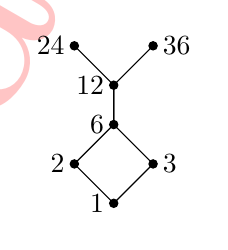
\begin{tikzpicture}[scale=0.5]
            \draw (0,-2) -- (1,-1) -- (0,0) -- (0,1) -- (1,2);
            \draw (0,-2) -- (-1,-1) -- (0,0) -- (0,1) -- (-1,2);
            \filldraw (0,-2) circle (3pt) node[left] {1};
            \filldraw (-1,-1) circle (3pt) node[left] {2};
            \filldraw (1,-1) circle (3pt) node[right] {3};
            \filldraw (0,0) circle (3pt) node[left] {6};
            \filldraw (0,1) circle (3pt) node[left] {12};
            \filldraw (-1,2) circle (3pt) node[left] {24};
            \filldraw (1,2) circle (3pt) node[right] {36};
      \end{tikzpicture}
      \end{center}
      }
\end{description}

\end{document} 